%!TEX root = ../template.tex
%%%%%%%%%%%%%%%%%%%%%%%%%%%%%%%%%%%%%%%%%%%%%%%%%%%%%%%%%%%%%%%%%%%%
%% chapter2.tex
%% NOVA thesis document file
%%
%% Chapter with the template manual
%%%%%%%%%%%%%%%%%%%%%%%%%%%%%%%%%%%%%%%%%%%%%%%%%%%%%%%%%%%%%%%%%%%%
\chapter{Estado-da-arte}
\label{cha:stateOfTheArt}
%{\LARGE \textbf{~\\These instructions are outdated! Please see also the “template.tex” file!\\}}
%
%This chapter describes how to use the \LaTeX\ \novathesis\ template (and the “\novathesisclass” class file).
%
%Let's start with some simple suggestions:
%
%\begin{enumerate}
%  \item No! You don't have to use this template to write your thesis.  You don't even have to use \LaTeX.  However, writing a thesis is serious stuff, and which tool you shall use to write it is not a decision to make lighthearted.
%  \item \LaTeX\ is hard enough by itself.  This template aims at making your life easier, but not easy. If you choose to use this template to write your thesis, you are very welcome.  However, don't expect me to provide you help with \LaTeX.  Look for help with your friends (you have some friends, don't you?), or search the web, or try even to read some book(s) on \LaTeX. In the end you will certainly find the experience rewarding.
%  \item So, don't forget, when you come to the point of “\emph{How do I do this with \LaTeX?}” look for help!  Google is your best friend. 
%  \item If you believe the difficulty is related with the \novathesis\ template itself (and not with \LaTeX), please \textbf{do not} send me an email asking for help.  Please look for help in the \novathesis\ Google Group (URL) and the \novathesis\ Facebook group (URL).  If you can't find help there from previous posts/messages, then post your own question. Hopefully someone will answer you.
%\end{enumerate}
%
%Now, let's go to a major issue for Windows users.  Characters have to be encoded in files as numbers, and that is how character encodings were born. ASCII and EBCDIC standards are long lost in the past.  The world now uses UTF-8.  Well, not all the world… Windows is still stick in its \emph{codepages}, and “latin1” is what windows uses as the codepage for Western Europe. This messes up with the template. Please be sure you use an editor with UTF-8 support.  \emph{Go to the preferences/options/… of your text editor and set up its default file encoding as UTF-8.}

% section introduction (end)
\section{GPU}
\label{gpus}


\section{Classificações de algoritmos}
\label{classi}
Com o passar do tempo cada vez mais algoritmos e respetivas adaptações para simular a docagem dos complexos de proteinas têm surgido, surgindo também formas de os classificar. Um algoritmo pode ser classificado em função da forma que trata a rigidez dos pares de proteinas a juntar ou até mesmo pelo modelo matemático, como por exemplo se aplicam a Fast Fourier Transform ou não.
Segundo o relatório de Huang Wenfan sobre o uso de Fast Fourier Transform associado à docagem de proteinas rigidas \cite{fftrigid}, existem três formas de se classificar um algoritmo de docagem, isto em relação às caracteristicas das proteinas em si, e não sobre o modelo matemático ou metodologias necessárias para o implementar:
\begin{itemize}
\item \textbf{Docagem Flexivel} Em que ambos os complexos receptor e ligando são considerados como sendo corpos flexiveis e adaptáveis sendo, no entanto, a mesma flexibidade interpretada pelo algoritmo de forma simplificada ou limitada, e por consequência pode-se aplicar um modelo através de simulações de docagem.
\item \textbf{Docagem Semi-Flexivel} Um dos corpos é considerado rigido e o outro não, em situações normais este tipo de algoritmos trata o ligando como se fosse a proteina flexivel, já que esta é mais pequena que a sua parceira, tendo assim uma maior probabilidade de mudar a sua forma, outra justificação tem a ver com os custos de computação serem mais baixos do que se considerarmos os receptores como flexiveis.
\item \textbf{Docagem Rigida} O par é considerado como sendo flexivel na sua integridade, sendo também considerado que na docagem entre os dois corpos uma das proteinas irá acabar por penetrar a outra o que leva a que se tenha de adaptar o conjunto de soluções para o problema em seis dimensões, 3 para a rotação e 3 para a translação.
\end{itemize}
Estes três conceitos são necessários para que se possa entender melhor os algoritmos nas secções seguintes, já que as suas complexidades dependem em certa forma da maneira como tratam a flexibilidade dos pares de proteinas e por consequência do número de dimensões que o espaço solução irá ter assim como a qualidade do conjunto solução encontrado.

\section{BiGGER}
\label{biggerAlg}
O algoritmo BiGGER (acrónimo para \textit{Bimolecular complex Generation with Global Evaluation and Ranking}) \cite{teseProf} de acordo com a classificação referida no ponto \ref{classi} enquadra-se no paradigma da docagem flexivel\cite{biggerPaper}
 permite resolver o problema de conseguir prever o ajuntamento dos complexos proteicos, 
consistindo essencialmente em dois passos, o primeiro efectua uma redução de possiveis configurações resultantes de passos de translação e rotação numa magnitude de cerca de $10^{15}$ configurações para milhares das anteriores isto através do algoritmo BoGIE relatado no ponto \ref{bogieAlg}. A segunda fase do algoritmo consiste em aplicar metodologias de aprendizagem automática de modo a que se possa prever qual das configurações resultantes corresponde ao melhor ajuste entre os dois complexos, isto é, a que tem o score mais elevado. Tal pode ser feito\\
Em termos de complexidade temporal, este algoritmo assume valores mais optimais ($O(N^(2.8))$\cite{biggerPaper}) do que os algoritmos que recorrem ao Fast Fourier Transform, estes últimos assumem como complexidade $O(N^{3}*log_2(N^{3}))$\cite{teseProf} e estes por sua vez têm uma melhor complexidade do que a dos algoritmos de correlação espacial ($O(N^6)$). O motivo pelo qual o das 3 especies de algoritmos o BiGGER assume-se com maior eficiencia em termos de computação deve-se ao facto de este ter sido implementado com diversas optimizações face aos algoritmos FFT, uma delas consiste no uso de uma heuristica mais eficiente no passo da eliminação de possibilidades: descarta situações em que existem sobreposições entre cores ou até mesmo situações que não cumprem com os limites impostos nas restrições \cite{biggerPaper}. \\
O tempo de computação, segundo os autores do algoritmo estava situado entre as 2H e as 8H, dependendo do par de proteinas, em contraste com o tempo de execução dos algoritmos FTT que ronda as 6H, com um CPU do ano de 2000 (Intel Pentium II 450 MHz dispoe apenas 1 core)\cite{biggerPaper}. Segundo a lei de moore, o número de transistors presentes num CPU duplica a cada 2 anos, e por consequencia a capacidade computacional. Num computador actual o tempo de execução do BiGGER provavelmente será menor, demorando entre 1H e 4H por exemplo, e após as paralelizações estarem concluidas espera-se que o algoritmo consiga efectuar as simulações num prazo de no máximo minutos.\\



\section{BoGIE}
\label{bogieAlg}
Acrónimo para \textit{Boolean Geometric Interaction Evaluation}\cite{teseProf} \cite{biggerPaper}, é um algoritmo de pesquisa em grelha utilizado na primeira fase do BiGGER, que é referido no ponto seguinte, mais precisamente na amostragem da população total de configurações possiveis para milhares, existem dois processos principais a considerar, sendo o primeiro a definição de uma matriz tridimensional de booleanos em que cada posição da matriz representa uma parcela da forma que o complexo assume, assume o valor1 se a celula corresponde a uma parcela da proteina cujo centro se encontra a uma distancia tri-dimensional que se designa por esfera de van der waals de qualquer outro átomo pertencente a outra proteina, as células com o valor 0 correspondem a frações do complexo que são consideradas como externas.\\
O segundo passo gera duas matrizes de boolean semelhantes às anteriores para cada um dos elementos do par: a matriz de superficie (\textit{surface matrix}) e a matriz central (\textit{core matrix}) tal como está ilustrado graficamente na figura \ref{fig:fig2subfig}. Os elementos celulares que ocupam a matriz de superficie são aqueles que na matriz inicial do passo anterior assumiram valor 1 mas tinham vizinhos com valor 0, ou seja, pretende-se os pontos de fronteira.\\ Na segunda matriz constam as células em que quer o seu valor, quer o das suas células vizinhas assumem valor verdadeiro o que corresponde a posições em que o seu centro está próximo do centro do complexo proteico ou podendo até mesmo coincidir. A forma de garantir que se consegue obter a superficie molecular da proteina é através da operação logica XOR (OU exclusivo), que terá como output 1 apenas nos pontos da fronteira, pois é aqui que o resultado do XOR associado aos dois pontos selecionados dá o valor verdadeiro, já que os valores entre as duas células são diferentes e falso se forem iguais.
Sendo assim  a complexidade deste algoritmo está associada mais com o primeiro passo do que com o segundo, já que este ultimo depende do output da matriz resultante do primeiro passo e apenas executa um conjunto de operações XOR o que não é assim tão custoso em termos de memória e tempo comparando com a medição para cada célula de uma distancia.
De notar, no entanto que ambos os passos podem ser optimizados recorrendo ao GPU, podendo trazer melhorias para além do uso do XOR.
\begin{figure}[htbp]
  \centering
    {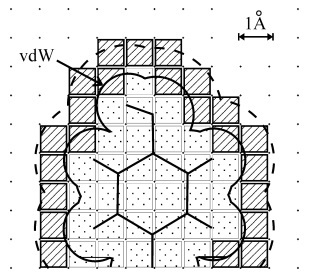
\includegraphics[width=0.5\linewidth]{figura1}}%
  \caption{Representação em 2D das matrizes resultantes do segundo passo do BoGIE, as células preenchidas a tracejado diagonal correspondem à matriz de superficie, as com pontos correspondem à matriz \textit{core} e a núvem com tracejado continuo representa o corte associado à esfera de van der waals com a proteina localizada ao centro \cite{biggerPaper}}
  \label{fig:fig2subfig}
\end{figure}

\section{Fast Fourier Transform}

\section{Algoritmos de correlação espacial}

%% ====================
%% = Folder Structure =
%% ====================
%\section{Folder Structure} % (fold)
%\label{sec:folder_structure}
%
%The \novathesis\ template is organized into files and folders. At the main level it includes the following files and folders:
%
%\noindent
%\begin{tabularx}{\linewidth}{>{\ttfamily}l>{\itshape}l>{\upshape}X}
%novathesis.cls     & file    & 
%The main class file. It will include additional files from \texttt{novathesis-files} folder. 
%\\ 
%template.tex      & file    & 
%The main user file. Use this file as the main file for your thesis. 
%\\
%bibliography.bib  & file    & 
%An example of a bibliography file. You may have has many as you want. \\
%template.pdf      & file    & 
%A possible result of applying pdf\LaTeX\ to the \texttt{template.tex} file. The template supports multiple types of documents (e.g., MSc dissertation, PhD thesis, …) and multiple Schools (e.g., FCT-NOVA, FCSH-NOVA, IST-UL, FC-UL, …) and each will produce different results.
%\\
%Chapters          & folder  & Examples of thesis chapters. Replace them with your own chapters. 
%\\
%Examples          & folder  & Some more examples of the use of the template for different document types and Schools. 
%\\
%Scripts           & folder  & Some (possibly useful) scripts for Unix-based systems (Linux, Mac OSx). If you are a windows user, ignore this folder (you may safely delete it if you want). 
%\\
%novathesis-files   & folder  & 
%Additional files for the \novathesisclass\ file.  Unless you know what you are doing, avoid messing up with the files and folders inside this folder (except for deleting the unused Schools, see below). 
%\\
%\end{tabularx}
%
%The \texttt{novathesis-files} folder contains additional files and folders that complement the main \novathesisclass\ file.  These are:
%
%\noindent
%\begin{tabularx}{\linewidth}{>{\ttfamily}l>{\itshape}l>{\upshape}X}
%README.txt      & file    &
%A file that should be read!  :) 
%\\
%fix-babel.clo   & file    &
%Simple fixes to the \texttt{babel} package.
%\\
%lang-text.clo   & file    &
%Translations of important strings used in the template.  Currently fully supported are Portuguese and English, but French is on the way.  If you add translations for your own language, please be so kind and send them to me. Thank you!
%\\
%options.clo     & file    &
%Processing of \novathesisclass\ options.  \emph{Don't mess with this!}
%\\
%packages.clo    & file    &
%Additional packages to be loaded into the \novathesis\ template. \emph{You should not mess with this!}
%\\
%spine.clo       & file    &
%This file is loaded only if the option \texttt{spine=true}, and includes the typesetting of the book spine.
%\\
%ChapStyles      & folder  &
%Contains a lot of files, one for each chapter style.  If you really know what you are doing, you may add your own chapter style here.
%\\
%FontStyles      & folder  &
%Contains a few files, one for each set of fonts (main text font, chapter font, section font, subsection font, etc).  If you really know what you are doing, you may add your own set here.
%\\
%Schools         & folder  &
%Configuration files for each school.  This folder is organized into subfolders, one for each university.  \emph{You may safely delete all the subfolders except the one for your University.}  Then open the subfolder of your University and \emph{you may safely delete all the subfolders except the one for your School/Faculty}.
%\\
%\end{tabularx}
%
%As stated above, the \texttt{Schools} folder contains per-university folders and per-school (faculty) subfolders.  Currently these are the available folders:
%
%\noindent
%\begin{tabularx}{\linewidth}{>{\ttfamily}r@{~/~}>{\ttfamily}l>{\itshape}l>{\upshape}X}
%ul     & ist    & folder  & 
%The folder for the \href{http://www.tecnico.ulisboa.pt}{\emph{Instituto Superior Técnico}} of the \emph{University of Lisbon}.
%\\
%nova    & fcsh   & folder  & 
%The folder for the \href{http:www.fcsh.unl.pt}{\emph{Faculty of Human and Social Sciences}}  of the \emph{NOVA University of Lisbon}.
%\\
%nova    & fct    & folder  & 
%The folder for the \href{http:www.fct.unl.pt}{\emph{Faculty of Sciences and Technology}} of the \emph{NOVA University of Lisbon}.
%\\
%nova    & novaims    & folder  & 
%The folder for the \href{http:www.novaims.unl.pt}{\emph{Information and Management School}} of the \emph{NOVA University of Lisbon}.
%\\
%\end{tabularx}

%% section folder_structure (end)
%
%% ===================
%% = Package options =
%% ===================
%\section{\novathesisclass\ Class Options} % (fold)
%\label{sec:package_options}
%
%The \novathesis\ class can be customized with the options listed below.
%
%\newcommand{\classoption}[3]{\textbf{#1=OPT}\qquad #2\\\qquad\emph{#3}\\}
%
%\noindent
%\begin{ctabular}{@{}p{\linewidth}@{}}
%  \toprule
%  \classoption{docdegree}%
%    {phd(*), phdplan, phdprop, msc, mscplan, bsc}%
%    {The type of the document: PhD Thesis (default), PhD Plan, PhD Proposal, MSc Disseration, MSc Plan, BSc Report}
%    \midrule
%  \classoption{school}%
%		{nova/fct(*), nova/fcsh, nova/ims, ul/ist, ul/fc}%
%    {The name of the school. This option changes the typesetting of the cover and some School specific formating, like margins, fonts, paragraph spacing and indentation, etc…}
%    \midrule
%  \classoption{lang}%
%    {en(*), pt}%
%    {The main language for the document.  Currently only Portuguese and English are supported.  Other languages are expected to be support in forthcoming versions.}
%    \midrule
%  \classoption{fontstyle}%
%    {bookman, charter, fourier, kpfonts(*), mathpazo1, mathpazo2, newcent}%
%    {The font set to be used in the document.  Please note that a font set include definitions for the main text, headings, maths, etc.}
%    \midrule
%  \classoption{chapstyle}%
%    {bianchi, bluebox, brotherton, dash, default, elegant(*), ell, ger, hansen, ist, jenor, lyhne, madsen, pedersen, veelo, vz14, vz34, vz43}%
%    {The chapter style, i.e., the look of the chapter beginning.}
%    \midrule
%  \classoption{converlang}%
%    {en, pt(*)}%
%    {The language to be used when typesetting the cover page.}
%    \midrule
%  \classoption{otherlistsat}%
%    {front(*), back}%
%    {Where to put the other lists besides the table of contents. The default is (\texttt{front}) before the main text.  But some scientific areas prefer them at the end of the document (\texttt{back}), just before the Appendixes.}
%    \midrule
%  \classoption{aftercover}%
%    {true, false(*)}%
%    {Include or don't include the contents of the “\texttt{aftercover}” file. The default is for this file to be ignored (if if it exists).}
%    \midrule
%  \classoption{linkscolor}%
%    {darkblue(*), black}%
%    {The color for all the hyperlinks in the PDF file.  The “\texttt{media=paper}” option (see below) will override this option to “\texttt{black}”}
%    \midrule
%  \classoption{spine}%
%    {true, false(*)}%
%    {Generate the book spine and the last page in the PDF.}
%    \midrule
%  \classoption{biblatex}%
%    {OPT=\{list of options for \texttt{biblatex}\}}%
%    {Customize \texttt{biblatex}, the bibliography management system used in this class. Probably you will want to change the value of the \texttt{biblatex} “\texttt{style}” option. For other customizations of \texttt{biblatex} check its manual.}
%    \midrule
%  \classoption{memoir}%
%    {OPT=\{list of options for \texttt{memoir}\}}%
%    {Customize the base class \texttt{memoir}. The \texttt{memoir} manual should be the first document to be consulted when looking for “\textbf{how can I do this?}” You may wnat to change the base font size from 11pt to a smaller (10pt) or larger (12pt) size.  Also, remember to change the “\texttt{draft}” to final when your document is finished.}
%    \midrule
%  \classoption{media}%
%    {screen(*), paper}%
%    {Behavior to be customized in the school options/configuration. Expected definitions for screen are: left and right margins are equal and use colored links. Expected definitions for paper are: left and right margins are different and use black links.}
%    \bottomrule
%\end{ctabular}
%
%\section{Additional considerations about the class options} % (fold)
%\label{sec:additional_considerations}
%
%In this section we will provide some additional considerations about some of the customizations available as class options.
%
%\subsection{The main language} % (fold)
%\label{sub:the_main_language}
%
%The choice of the main language with the option “\texttt{lang=OPT}” affects:
%
%\begin{itemize}
%	\item \textbf{The order of the summaries.} First is printed the abstract in the main language and then in the foreign language. This means that if your main language for the document in English, you will see first the “abstract” (in English) and then the “resumo” (in Portuguese). If you switch the main language for the document for Portuguese, it will also automatically switch the order of the summaries to “resumo” and then “abstract”.
%	\item \textbf{The names for document sectioning.} E.g., ``Chapter'' vs.\ ``Capítulo'', ``Table of Contents'' vs.\ ``Índice'', ``Figure'' vs.\ ``Figura'', etc.
%	\item \textbf{The type of documents in the bibliogrpahy.} E.g., ``Technical Report'' vs.\ ``Relatório Técnico'', ``PhD Thesis'' vs.\ ``Tese de Doutoramento'', etc.
%\end{itemize} 
%
%No mater which language you chose, you will always have the appropriate hyphenation rules according to the language at that point. You always get Portuguese hyphenation rules in the ``Resumo'', english hyphenation rules in the ``Abstract'', and then the main language hyphenation rules for the rest of the document.
%
%% subsection the_main_language (end).
%
%% section additional_consideration (end)
%
%
%\subsection{Class of Text} % (fold)
%\label{sub:class_of_text}
%
%You must choose the class of text for the document. The available options are:
%
%\begin{enumerate}
%	\item \textbf{bsc} --- BSc graduation report.
%	\item \textbf{*mscplan} --- Preparation of MSc dissertation. This is a preliminary report graduate students at DI-FCT-NOVA must prepare to conclude the first semester of the two-semesters MSc work. The files specified by \verb!\dedicatoryfile! and \verb!\acknowledgmentsfile! are ignored, even if present, for this class of document.
%	\item \textbf{msc} --- MSc dissertation.
%	\item \textbf{phdprop} ---  Proposal for a PhD work. The files specified by \verb!\dedicatoryfile! and \verb!\acknowledgmentsfile! are ignored, even if present, for this class of document.
%	\item \textbf{prepphd} ---  Preparation of a PhD thesis. This is a preliminary report PhD students at DI-FCT-NOVA must prepare before the end of the third semester of PhD work. The files specified by \verb!\dedicatoryfile! and \verb!\acknowledgmentsfile! are ignored, even if present, for this class of document.
%	\item \textbf{phd} --- PhD dissertation.
%\end{enumerate}
%% subsection class_of_text (end)
%
%% ============
%% = Printing =
%% ============
%\subsection{Printing} % (fold)
%\label{sub:printing}
%
%You must choose how your document will be printed. The available options are:
%\begin{enumerate}
%	\item \textbf{oneside} --- Single side page printing.
%	\item \textbf{*twoside} --- Double sided page printing.
%\end{enumerate}
%% subsection printing (end)
%
%% =============
%% = Font Size =
%% =============
%\subsection{Font Size} % (fold)
%\label{ssec:font_size}
%
%You must select the encoding for your text. The available options are:
%\begin{enumerate}
%	\item \textbf{11pt} --- Eleven (11) points font size.
%	\item \textbf{*12pt} --- Twelve (12) points font size. You should really stick to 12pt\ldots
%\end{enumerate}
%% subsection font_size (end)
%
%% =================
%% = Text encoding =
%% =================
%\subsection{Text Encoding} % (fold)
%\label{ssec:text_encoding}
%
%You must choose the font size for your document. The available options are:
%\begin{enumerate}
%	\item \textbf{latin1} --- Use Latin-1 (\href{http://en.wikipedia.org/wiki/ISO/IEC_8859-1}{ISO 8859-1}) encoding.  Most probably you should use this option if you use Windows;
%	\item \textbf{utf8} --- Use \href{http://en.wikipedia.org/wiki/UTF-8}{UTF8} encoding.    Most probably you should use this option if you are not using Windows.
%\end{enumerate}
% subsection font_size (end)

% ============
% = Examples =
% ============
%\subsection{Examples} % (fold)
%\label{ssec:examples}
%
%Let's have a look at a couple of examples:
%
%\begin{itemize}
%	\item Preparation of PhD thesis, in portuguese, with 11pt size and to be printed single sided (I wonder why one would do this!)\\
%	\verb!\documentclass[prepphd,pt,11pt,oneside,latin1]{thesisdifct-nova}!
%	\item MSc dissertation, in english, with 12pt size and to be printed double sided\\
%	\verb!\documentclass[msc,en,12pt,twoside,utf8]{thesisdifct-nova}!
%\end{itemize}
%% subsection examples (end)
%
%\section{How to Write Using \LaTeX} % (fold)
%\label{sec:how_to_write_using_latex}
%
%Please have a look at Chapter~\ref{cha:a_short_latex_tutorial_with_examples}, where you may find many examples of \LaTeX constructs, such as Sectioning, inserting Figures and Tables, writing Equations, Theorems and algorithms, exhibit code listings, etc.
%
%% section how_to_write_using_latex (end)
%
%
%
%\section{Exmaple glossary and acronyms}
%%
%% \todo[inline]{A a note in a line by itself.}
%%
%This is the first occurrence of an abbreviation: \gls{abbrev}. And now the second occurrence of the same abbreviation: \gls{abbrev}. And a new acronym with capital letter: \Gls{xpt} and reused \gls{xpt}.  Let's also use a few other acronyms such as \gls{aaa}, \gls{aab}, \gls{aba}, \gls{bbb} and \gls{xpt}.
%
%
%Lets add the term ``\gls{computer}'' to the glossary!
%
% Please note that
% \begin{center}
%   \textbf{\large this package and template are not official for FCT/NOVA}.
% \end{center}
